\documentclass{article}

\usepackage{fullpage}
\usepackage{graphicx}
\usepackage{color}
\usepackage{fancyhdr}
\usepackage{url}
\usepackage{amsmath,bm}
\usepackage{amssymb}
\usepackage{amsthm}
\usepackage{amsfonts}
\usepackage[round]{natbib}
\usepackage{enumitem,xcolor}
\usepackage[multiple]{footmisc}

\usepackage[
 pdftitle={Capstone Proposal - Udacity Machine Learning Nanodegree},
 pdfsubject={Machine Learning, Reinforcement Learning, Deep Learning, Artificial Intelligence, Games},
 pdfauthor={Peng Xu},
 pdfpagemode=UseOutlines,
 pdfborder= {0 0 1.0},
 bookmarks,
 bookmarksopen,
 colorlinks=true,
 citecolor=blue,
 linkcolor=blue, %
 linkbordercolor=blue, %
 urlcolor=blue, %
]{hyperref}

\usepackage[labelfont=bf]{caption}


\usepackage[utf8]{inputenc}

% Default fixed font does not support bold face
\DeclareFixedFont{\ttb}{T1}{txtt}{bx}{n}{8} % for bold
\DeclareFixedFont{\ttm}{T1}{txtt}{m}{n}{8}  % for normal

% Custom colors
\usepackage{color}
\definecolor{deepblue}{rgb}{0,0,0.5}
\definecolor{deepred}{rgb}{0.6,0,0}
\definecolor{deepgreen}{rgb}{0,0.5,0}

\usepackage{listings}

\definecolor{codebg}{RGB}{238,238,238}

% Python style for highlighting
\newcommand\pythonstyle{\lstset{
language=Python,
basicstyle=\ttm,
otherkeywords={self},             % Add keywords here
keywordstyle=\ttb\color{deepblue},
emph={MyClass,__init__},          % Custom highlighting
emphstyle=\ttb\color{deepred},    % Custom highlighting style
stringstyle=\color{deepgreen},
frame=tb,                         % Any extra options here
framesep=10pt,
framexleftmargin=10pt,
backgroundcolor=\color{codebg},
rulecolor=\color{codebg},
aboveskip=15pt,
belowskip=15pt,
showstringspaces=false            % 
}}


% Python environment
\lstnewenvironment{python}[1][]
{
\pythonstyle
\lstset{#1}
}
{}

% Python for external files
\newcommand\pythonexternal[2][]{{
\pythonstyle
\lstinputlisting[#1]{#2}}}

% Python for inline
\newcommand\pythoninline[1]{{\pythonstyle\lstinline!#1!}}

\graphicspath{ {../images/} }

%%%%%%%%%%%%%%%%%%%%%%%%%%%%%%%%%%%%%%%%%%%%%%%%%%%%%%%%%%%%%%%%%%%%%%%%%%%%%%%%%%%%%%%%%%%%%%%%%%%%
\title{Machine Learning Nanodegree \\ Capstone Proposal}
\author{Peng Xu}
\date{February 13, 2016}
\begin{document}
\maketitle
%%%%%%%%%%%%%%%%%%%%%%%%%%%%%%%%%%%%%%%%%%%%%%%%%%%%%%%%%%%%%%%%%%%%%%%%%%%%%%%%%%%%%%%%%%%%%%%%%%%%

%%%%%%%%%%%%%%%%%%%%%%%%%%%%%%%%%%%%%%%%%%%%%%%%%%%%%%%%%%%%%%%%%%%%%%%%%%%%%%%%%%%%%%%%%%%%%%%%%%%%
\section{Domain Background}
%%%%%%%%%%%%%%%%%%%%%%%%%%%%%%%%%%%%%%%%%%%%%%%%%%%%%%%%%%%%%%%%%%%%%%%%%%%%%%%%%%%%%%%%%%%%%%%%%%%%

Reinforcement learning addresses the problem of how agents should learn to take actions to maximize cumulative reward through interactions with the environment. The traditional approach for reinforcement learning algorithms requires carefully chosen feature representations, which are usually hand-engineered. Recently, significant progress has been made by combining advances in deep learning for learning feature representations.

Deep Reinforcement Learning has proven its ability in a varity of classic problems among video games and robotics. In some extent, a video game is equivelent to a simulation of real case, such as racing cars, drones etc. By solving a similar problem in a video game or a simulation setting, the final successful model could be applied on the countpart problem in real case using transfer learning, which saves a lot of time and money or even reverse mission impossible. Among those challenging problems how to train a vehicle to be a self-learner interests me most.

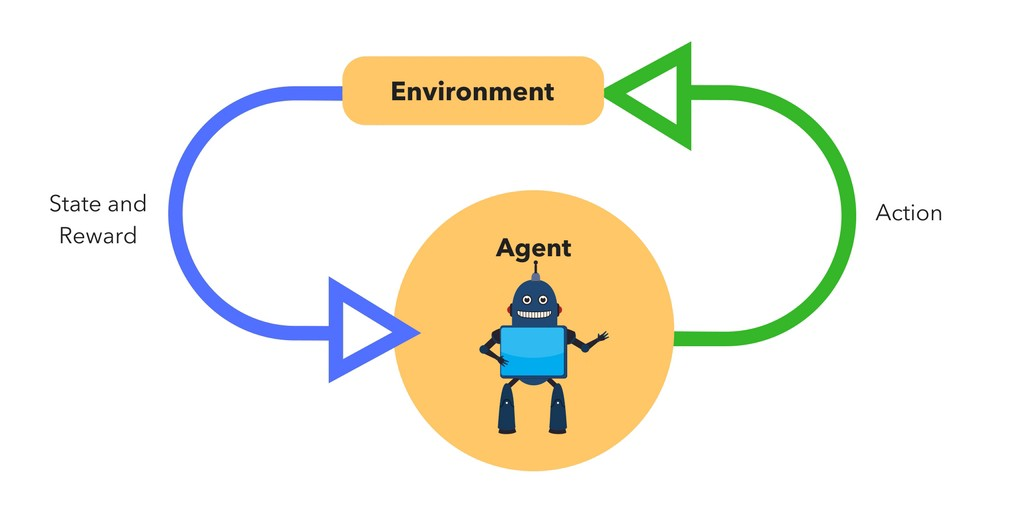
\includegraphics[width=\textwidth]{interaction-flow}

In other words, a general pipeline is to be established along with this practice of building a game bot. In the future, the pipeline could be applied on similar problems both in simulation setting and in field cases which is the motivation for me.

%%%%%%%%%%%%%%%%%%%%%%%%%%%%%%%%%%%%%%%%%%%%%%%%%%%%%%%%%%%%%%%%%%%%%%%%%%%%%%%%%%%%%%%%%%%%%%%%%%%%
\section{Problem Statement}
\label{sec:problem-statement}
%%%%%%%%%%%%%%%%%%%%%%%%%%%%%%%%%%%%%%%%%%%%%%%%%%%%%%%%%%%%%%%%%%%%%%%%%%%%%%%%%%%%%%%%%%%%%%%%%%%%

\newcommand{\URLcf}{https://en.wikipedia.org/wiki/Connect_Four}

In openAI-Universe, several racing car games are provided, for example, the Coaster Racer flash game, in which a vehicle is simply controlled by 3 inputs, left, right, forward. It is easily to be redesigned in a Reinoforcement Learning setting. The vehicle interacts with its environment in the way as shown in below. It is expected that the racing car can learn a smart driving behavior after a series of training steps leading to a maximal reward or namely score here.

This is starting from the "How to Install OpenAI's Universe and Make a Game Bot" live session by Siraj Raval on Youtube. The bot is for the Coaster Racer flash game and determines the answer to 2 questions -- should I turn, and which way should I turn? It answers the first by checking if it's been receiving a reward for a certain interval (no crashes), and if it has it will turn. It answers the second by randomly picking a turn between left and right. This bot is able to complete the race. So it's a bot that uses reinforcement learning to determine when to turn and each turn is a random direction.

\begin{itemize}

    \item \textbf{Task:} Playing Coaster Racer.

    \item \textbf{Performance:} Percent of games won against other agents.

    \item \textbf{Experience:} Games played against itself.

    \item \textbf{Target function:} $Q^\pi : \mathcal{S} \times \mathcal{A} \to \mathbb{R}$, where
        $\mathcal{S}$ is the set of \emph{states} (board positions) and $\mathcal{A}$ is the set of
        \emph{actions} (moves), and $\mathbb{R}$ represents the value of being in a state $s \in
        \mathcal{S}$, applying a action $a \in \mathcal{A}$, and following policy $\pi$ thereafter.

    \item \textbf{Target function representation:} Deep neural network.

\end{itemize}

Therefore, I seek to build a Q-learning agent trained via a deep convolutional neural network to
approximate the optimal action-value function:

\begin{equation}
Q^*(s,a) = \max\limits_\pi Q^\pi(s,a), \forall s \in \mathcal{S}, a \in \mathcal{A}
\end{equation}

\noindent which is the maximum sum of rewards achievable by a behaviour policy $\pi$.

%%%%%%%%%%%%%%%%%%%%%%%%%%%%%%%%%%%%%%%%%%%%%%%%%%%%%%%%%%%%%%%%%%%%%%%%%%%%%%%%%%%%%%%%%%%%%%%%%%%%
\section{Datasets and Inputs}
%%%%%%%%%%%%%%%%%%%%%%%%%%%%%%%%%%%%%%%%%%%%%%%%%%%%%%%%%%%%%%%%%%%%%%%%%%%%%%%%%%%%%%%%%%%%%%%%%%%%

By using a Deep Q-Learning model, there is no need to use an external dataset since the data are captured along with training. 

%%%%%%%%%%%%%%%%%%%%%%%%%%%%%%%%%%%%%%%%%%%%%%%%%%%%%%%%%%%%%%%%%%%%%%%%%%%%%%%%%%%%%%%%%%%%%%%%%%%%
\section{Solution Statement}
%%%%%%%%%%%%%%%%%%%%%%%%%%%%%%%%%%%%%%%%%%%%%%%%%%%%%%%%%%%%%%%%%%%%%%%%%%%%%%%%%%%%%%%%%%%%%%%%%%%%

To tackle the problem described in \hyperref[sec:problem-statement]{Section
\ref*{sec:problem-statement}}, we will use Reinforcement learning with Deep Learning to
automatically learn evaluation functions by playing games by itself. Unlike other approaches
that need a very large dataset, this approach will try to learn to play games without any domain
knowledge (no dataset will be used). This is a promising approach for creating game-playing
algorithms for playing other two-player games of perfect information.

%%%%%%%%%%%%%%%%%%%%%%%%%%%%%%%%%%%%%%%%%%%%%%%%%%%%%%%%%%%%%%%%%%%%%%%%%%%%%%%%%%%%%%%%%%%%%%%%%%%%
\section{Benchmark Model}
\label{sec:benchmark}
%%%%%%%%%%%%%%%%%%%%%%%%%%%%%%%%%%%%%%%%%%%%%%%%%%%%%%%%%%%%%%%%%%%%%%%%%%%%%%%%%%%%%%%%%%%%%%%%%%%%

\begin{itemize}

    \item \textbf{Random agent}. This benchmark consists in playing against an agent that takes
        uniformly random moves. This is the most basic benchmark, but first we have to be sure that
        our learned evaluation function can play better than a random agent before moving into a
        harder benchmark. Also, this will help us to detect bugs in the code and algorithms: if a
        learned value function does not play significantly better than a random agent, is not
        learning. The idea is to test against this benchmark using Alpha-beta pruning at 1, 2 and
        4-ply search.

\end{itemize}

%%%%%%%%%%%%%%%%%%%%%%%%%%%%%%%%%%%%%%%%%%%%%%%%%%%%%%%%%%%%%%%%%%%%%%%%%%%%%%%%%%%%%%%%%%%%%%%%%%%%
\section{Evaluation Metrics}
%%%%%%%%%%%%%%%%%%%%%%%%%%%%%%%%%%%%%%%%%%%%%%%%%%%%%%%%%%%%%%%%%%%%%%%%%%%%%%%%%%%%%%%%%%%%%%%%%%%%

\begin{itemize}

    \item \textbf{Winning percentage.} This metric consists in playing a high number of games (e.g.
        100,000) against another agent (e.g. a random agent), and calculating the average of games
        won by the agent that uses the learned value function.

\end{itemize}

%%%%%%%%%%%%%%%%%%%%%%%%%%%%%%%%%%%%%%%%%%%%%%%%%%%%%%%%%%%%%%%%%%%%%%%%%%%%%%%%%%%%%%%%%%%%%%%%%%%%
\section{Project Design}
\label{sec:project-design}
%%%%%%%%%%%%%%%%%%%%%%%%%%%%%%%%%%%%%%%%%%%%%%%%%%%%%%%%%%%%%%%%%%%%%%%%%%%%%%%%%%%%%%%%%%%%%%%%%%%%

%%%%%%%%%%%%%%%%%%%%%%%%%%%%%%%%%%%%%%%%%%%%%%%
\subsection{Programming Language and Libraries}
%%%%%%%%%%%%%%%%%%%%%%%%%%%%%%%%%%%%%%%%%%%%%%%

\begin{itemize}

    \item \textbf{Python 2.}

    \item \textbf{openai-gym}. Open source machine learning library for Reinforcement Learning.
    
    \item \textbf{openai-universe}. Provide the game environment.

    \item \textbf{Keras.} Open source neural network library written in Python. It is capable of
        running on top of either Tensorflow or Theano.

    \item \textbf{TensorFlow.} Open source software libraries for deep learning.

\end{itemize}

%%%%%%%%%%%%%%%%%%%%%%%%%%%%%%%%%%%%
\subsection{Environments and Agents}
%%%%%%%%%%%%%%%%%%%%%%%%%%%%%%%%%%%%

\begin{itemize}

    \item \textbf{Coaster Racer flash game.} Will be used to verify that the reinforcement learning algorithms
        are working as expected, since it is a simple game where an agent can easily search the full
        game tree to find the optimal actions.

\end{itemize}

%%%%%%%%%%%%%%%%%%%%%%%%%%%%%%%%%%%%
\subsection{Machine Learning Design}
%%%%%%%%%%%%%%%%%%%%%%%%%%%%%%%%%%%%

\begin{itemize}

    \item \textbf{Type of training experience:} Games against self

    \item \textbf{Target function:} $Q^\pi : \mathcal{S} \times \mathcal{A} \to \mathbb{R}$, where
        $\mathcal{S}$ is the set of \emph{states} (board positions) and $\mathcal{A}$ is the set of
        \emph{actions} (moves), and $\mathbb{R}$ represents the value of being in a state $s \in
        \mathcal{S}$, applying a action $a \in \mathcal{A}$, and following policy $\pi$ thereafter.

    \item \textbf{Representation of learned function:} Deep neural network

    \item \textbf{Learning algorithm:} Q-learning, a model-free online off-policy algorithm, whose
        main strength is that it is able to compare the expected utility of the available actions
        without requiring a model of the environment:

        \begin{equation}
        Q(s_t, a_t) \gets Q(s_t, a_t) + \alpha [r_{t+1} + \gamma \max_a Q(s_{t+1}, a) - Q(s_t, a_t)]
        \end{equation}


\end{itemize}

%%%%%%%%%%%%%%%%%%%%%%%%%%%%%%%%%%%%%%%%%%%%%%%%%%%%%%%%%%%%%%%%%%%%%%%%%%%%%%%%%%%%%%%%%%%%%%%%%%%%
% BIBLIOGRAPHY
%%%%%%%%%%%%%%%%%%%%%%%%%%%%%%%%%%%%%%%%%%%%%%%%%%%%%%%%%%%%%%%%%%%%%%%%%%%%%%%%%%%%%%%%%%%%%%%%%%%%

\bibliographystyle{plainnat}
\bibliography{bibliography}

\end{document}